\vorlesung{26. Oktober bis 17. November 2017}
\chapter{Grundelemente der Teilchenphysik}
\section{Fundamentale Bausteine der Materie}
Heute: Materie besteht aus wenigen elementaren Teilchen (Spin $cefrac{1}{2}$, Fermionen)
\begin{align*}\begin{matrix}
\text{Leptonen }& \begin{pmatrix} \nu_e \\ e^- \end{pmatrix}& \begin{pmatrix} \nu_\mu \\ \mu^- \end{pmatrix}&\, \begin{pmatrix} \nu_\tau \\ \tau^- \end{pmatrix} & \\
& & & & + \text{ Antiteilchen} \\
\text{Quarks }& \underbrace{\begin{pmatrix} u \\ d \end{pmatrix}}_{1.\text{Gen.}} & \, \underbrace{\begin{pmatrix} c \\ s \end{pmatrix}}_{2.\text{Gen.}} &\, \underbrace{\begin{pmatrix} t \\ b \end{pmatrix}}_{3.\text{Gen.}} & 
\end{matrix}
\end{align*}
\begin{itemize}
\item geladene Leptonen: $e$ (Elektron), $\mu$ (Myon), $\tau$ (Tauon)
\item neutrale Leptonen (Neutrinos): $\nu_e$, $\nu_\mu$, $\nu_\tau$ 
\item Quarks: up, down, charm, strange, top, bottom
\item[$\ra$] Quarks treten \tb{nie} als freie Teilchen auf, sondern in gebundenen Systemen: $p, \ n, \ \pi$
\item[$\ra$] Alle Leptonen und Quarks sind \glqq punktförmig\grqq: Experiment $<\, 10^{-18}$\,m
\end{itemize}
\subsection{Massen und Ladungen}
\begin{center}
\begin{tabular}{l | c | c}
Teilchen & Masse & Ladung [$e$]\\
\hline
Elektron $e^-$ & 511\,keV & -1 \\
Myon $\mu^-$ & 106\,MeV & -1\\
Tau $\tau^-$ & 1777\,MeV & -1\\
e-Neutrino $\nu_e$ & < 2.2\,eV & 0\\
$\mu$-Neutrino $\nu_\mu$ & < 0.17\,MeV & 0\\
$\tau$-Neutrino $\nu_\tau$ & < 15.5\, MeV & 0\\
up-Quark $u$ & 1.5 - 3.3\,MeV & $+cefrac{2}{3}$\\
charm-Quark $c$ & 1.27\,GeV & $+cefrac{2}{3}$\\
top-Quark $t$ & 177\,GeV & $+cefrac{2}{3}$\\
down-Quark $d$ & 3.5 - 6\,MeV & $-cefrac{1}{3}$\\
strange-Quark $s$ & 104\,MeV & $-cefrac{1}{3}$\\
bottom-Quark $b$ & 4.2\,GeV & $-cefrac{1}{3}$
\end{tabular}
\end{center}
\begin{itemize}
\item \tb{Antiteilchen}: Zu jedem Teilchen $T$ existiert ein Antiteilchen $\bar{T}$ mit Spin$\lb \bar{T}\rb $ = Spin($T$), \newline Masse$\lb \bar{T}\rb $ = Masse$\lb T\rb $,  und Ladung$\lb \bar{T}\rb $ = $-$ Ladung$\lb T\rb $
\begin{itemize}
\item[$\ra$] Erstes experimentell gefundenes Antiteilchen: Positron $e^+$
\item[$\ra$] Antiteilchen können Antimaterie bilden (Bsp.: Anti-H = $\bar{p} +e^+$)
\item[$\ra$] Urknall: Gleiche Menge Materie/Antimaterie (Wieso sehen wir Materie?)
\end{itemize}
\end{itemize}
\section{Fundamentale Kräfte (Wechselwirkungen)}
Für Teilchen ist \glqq Kraftfeld\grqq{} keine geeignete Beschreibung
\begin{compactitem}
\item[$\ra$] Quantenmechanik 
\item[$\ra$] keine wohldefinierte Trajektorie
\item[$\ra$] keine Teilchenumwandlung
\end{compactitem}
\tb{Lösung:}\\
Quantisiere Kraftfeld $\ra$ \tb{Quantenfeldtheorie}\\
Teilchen-Wechselwirkung $\hat{=}$ Austausch von Feldquanten $\ra$ Übertragung von Energie und Impuls

\tb{Fundamentale Wechselwirkungen}
\begin{center}
\begin{tabular}{l | l | c | c}
Wechselwirkung & Partner & Quant & Stärke \\
\hline
elektromagnetische WW & geladene Teilchen & $\gamma$ =  Photon & $\sim$ Ladung\\
schwache WW & alle Fermionen & $W^\pm$, $Z^0$ & schwach\\
starke WW & Quarks & $g$ = Gluon & $\sim$ starke Ladung \\
Gravitation & alle Teilchen & ? & i.A. vernachlässigbar
\end{tabular}
\end{center}
\begin{compactitem}
\item[$\ra$] Massen: $m_\gamma = m_g = 0$, $M_{W^\pm} \approx 80.4\,$GeV, $M_{Z^0} \approx 91.2$\,GeV
\item[$\ra$] Alle haben Spin 1
\item[$\ra$] Gluon trägt Farbladung $\Ra$ massive Auswirkung auf Phänomenologie der starken WW
\end{compactitem}
\section{Feynman-Diagramme}
Beschreibung von Wechselwirkungen (z.B. $e^-e^- \ra e^-e^-$)
\begin{center}
\captionsetup{type=figure}
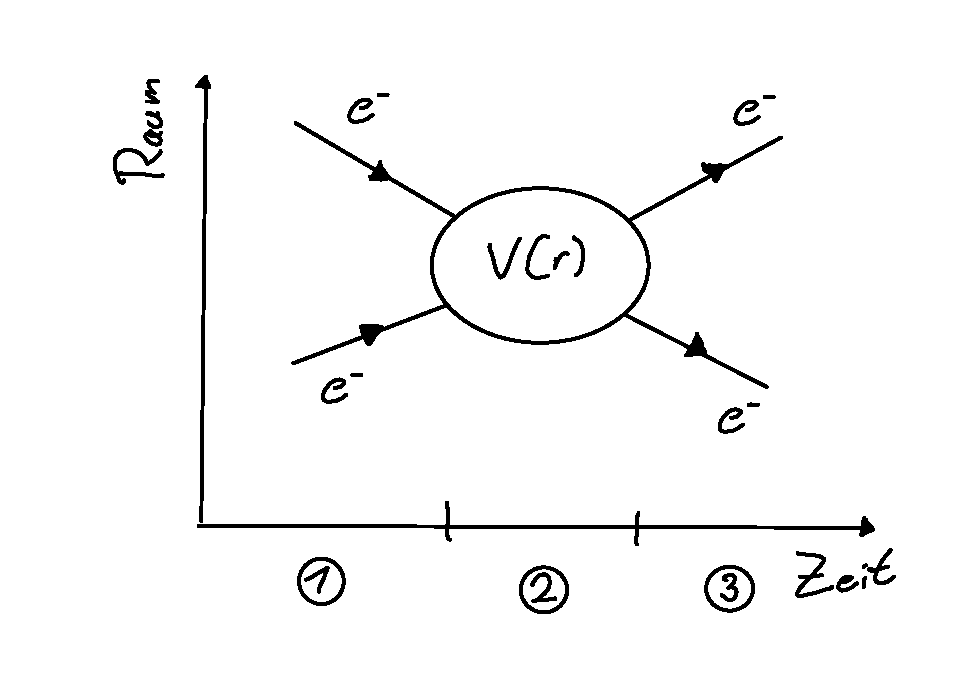
\includegraphics[width=.5\textwidth]{imgs/ep5-fig-2-1.pdf}
\captionof{figure}{Schematisch-allgemeine Darstellung eines Feynmandiagramms (Achtung, die Ausdehnung von $V(r)$ kann unendlich sein)\label{fig:2.1}}
\end{center}
\begin{compactitem}
\item[1.] Anfangszustand: \glqq freie\grqq{} Teilchen $\ra$ ebene Wellen
\item[2.] WW durch WW-Potential $\ra$ Störung der ebenen Wellen\\
beschrieben durch Störungsreihe der Quantenfeldtheorie (QFT)
\begin{compactitem}
\item[$\ra$] ungestörtes System: Teilchen \glqq merken nichts voneinander\grqq
\item[$\ra$] Niedrigste Ordnung der Störung: Austausch eines WW-Quants
\item[$\ra$] Höhere Ordnungen: mehrere Quanten ausgetauscht
\end{compactitem}
\item[3.] Endzustand: \glqq freie\grqq{} Teilchen $\ra$ ebene Welle
\end{compactitem}
Elemente der Störungsreihe dargestellt durch Feynman-Diagramme

\tb{1. Ordnung (Bsp.: $e^-e^- \ra e^-e^-$)}
\begin{compactitem}
\item Jedes FD symbolisiert eindeutige Rechenvorschrift für Übergangsmatrixelement ($\ra$ QFT)
\item An jedem Vertex erhalten:
\begin{compactitem}
\item Energie, Impuls
\item Ladung
\item Leptonzahl $L = N(L) - N\lb \bar{L}\rb $
\end{compactitem}
\end{compactitem}
\begin{figure}[!ht]
\centering
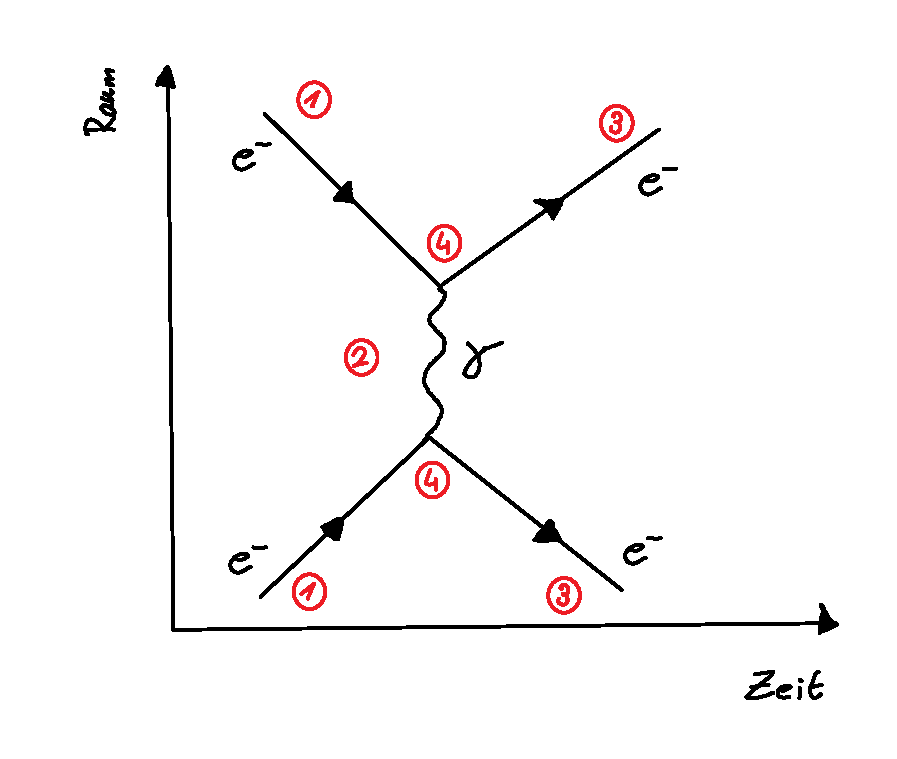
\includegraphics[width=.5\textwidth]{imgs/ep5-fig-2-2.pdf}
\caption{Feynman-Diagramm, 1: einlaufende Fermionen, 2: Austausch-Quant, 3: auslaufende Fermionen, 4: Vertex = Kopplung zwischen Quant-Fermionen\label{fig:2.2}}
\end{figure}

\noindent \tb{Energie- und Impulsübertrag am Vertex (vgl. Abb.\ref{fig:2.3})}\\
\begin{figure}[!ht]
\centering
\begin{tikzpicture}
    \begin{feynman}
    \vertex (a1);
    \vertex [below right = 2cm of a1] (b1);
    \vertex [above right = 2cm of b1] (a2);
    \vertex [below = 2cm of b1] (c1);
    
    \diagram*{
    (a1) -- [fermion, edge label' = $e^-(p)$] (b1) -- [fermion, edge label' = $e^-\left( p'\right)$] (a2),
    (b1) -- [photon, edge label = $\gamma$] (c1),
    };
    \end{feynman}
\end{tikzpicture}
\caption{Schematische Darstellung der Übertragung, hier für elektrodynamische Wechselwirkung \label{fig:2.3}}
\end{figure}
\begin{align}
p_\mu, \, p^\prime_\mu,\, q_\mu : \text{4er-Impulse mit } q_\mu = p_\mu - p^\prime_\mu
\end{align}
\newpage
\tb{Elastische Streuung im CMS:}
\begin{align}
\begin{split}
E = E^\prime & \Ra q_\mu = \lb  0, \vec{p} -\vec{p}\prime \rb \\
 & \Ra q^2_\mu = q_\mu q^\mu = \underbrace{-\lb \vec{p} - \vec{p}^\prime\rb ^2}_{<0!}
\end{split}
\end{align}
\begin{compactitem}
\item[$\Ra$] $E_\gamma$, $\vec{p}_\gamma$ \glqq passen nicht\grqq{} zu Photon mit Masse 0
\item[$\Ra$] Austauschteilchen ist \glqq virtuell\grqq{} bzw. \glqq off-mass-shell\grqq{} $\hat{=}$ QFT-Feldanregungen, die \tb{nicht} als eigenständige Teilchen propagieren können
\item[$\Ra$] Austauschteilchen nicht sichtbar/messbar
\end{compactitem}
\tb{Quantitative Elemente}
\begin{itemize}
\item \tb{Vertex}\\
Für elektromagnetische WW-Kopplungsstärke $\sim$ elmag. Ladung ($Z\cdot e$)\\
Andere Wechselwirkungen haben andere Ladungen
\item \tb{Austauschteilchen}
\begin{align}
\boxed{\text{Propagator} \sim \frac{1}{q^2-m^2}}
\end{align}
mit Impuls $q$ und Masse $m$ des Austauschteilchens. Umso kleiner der Propagator, desto \glqq virtueller\grqq{} das Austauschteilchen.\\
Für $\gamma: \, m_\gamma =0$ $\ra$ Propagatorterm $\sim \frac{1}{q^2}$
\item \tb{Matrixelement}\\
Die Matrix $M$ lässt sich berechnen mit Anfangszustand $i$, Endzustand $f$ und Wechselwirkungshamiltonian $\Ham_{WW}$:
\begin{align}
M = \lla f\labs  \Ham_{WW} \rabs  i \rra
\end{align}
Es gilt also
\begin{align*}
M \sim \lb  \text{Kopplungsstärke}\rb _\text{Vertex1} \times \text{Propagator} \times \lb  \text{Kopplungsstärke}\rb _\text{Vertex2}
\end{align*}
Die Reaktionswahrscheinlichkeit ergibt sich zu $\sim \labs M\rabs^2$\\
\tb{Beispiel:} $e^-e^- \ra e^-e^-$
\begin{align}
\labs M \rabs^2 = \labs e \cdot \frac{1}{q^2} \cdot e \rabs^2 = \frac{e^4}{q^4} \sim \frac{\alpha^2}{q^4}
\end{align}
mit $\alpha$: Feinstrukturkonstante\\
$\ra$ $\alpha$ ist Maß für Stärke der WW
\begin{align}
\begin{split}
\ra q^2 = - \lb  \vec{p} - \vec{p}^\prime \rb ^2 \overset{\labs\vec{p}\rabs = \labs \vec{p}^\prime\rabs}{=} -2p^2 +2p^2\cos \vartheta = -4 p^2 \sin^2 \lb \frac{\vartheta}{2}\rb \\
\Ra \boxed{\labs M \rabs^2 \sim \frac{1}{\sin^4 \lb \frac{\vartheta}{2}\rb }}\\
\text{ Kleinwinkelstreuung dominiert}
\end{split}
\end{align}
\item \tb{Höhere Ordnung} (vgl. Abb.\ref{fig:2.4})\\
$ M = \sum\limits_n M_{n,i}$ mit $i=$ Beuträge zur Ordnung $n$
Für 1. Ordnung ist $\labs M \rabs ^2 \sim \alpha^2$, für 2. Ordnung $\labs M \rabs ^2 \sim \alpha^4$
\begin{compactitem}
\item[$\ra$] Interferenz: $\labs M \rabs ^2 \sim \alpha^3$
\item[$\ra$] Störungsreihe konvergiert gut $\alpha \ll 1$
\item[$\ra$] Achtung: Höhere Ordnungen enthalten \glqq Loops\grqq{} und erfordern besondere theoretische Behandlung (Stichwort: \glqq Renormierung\grqq)
\end{compactitem}
\begin{figure}[!ht]
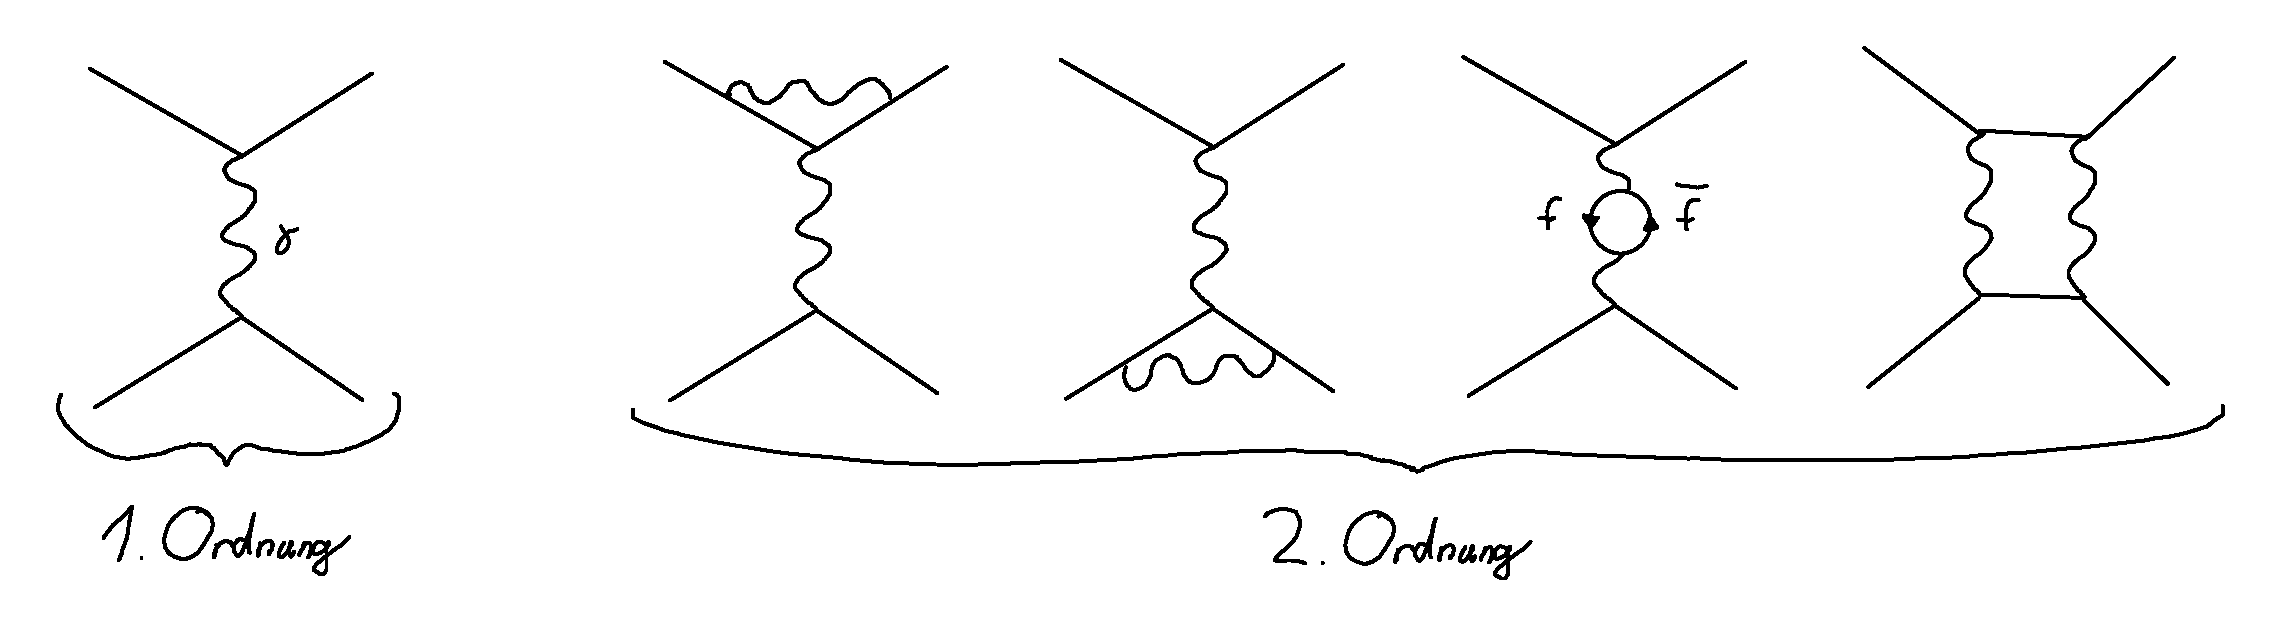
\includegraphics[width=\textwidth]{imgs/ep5-fig-2-4.pdf}
\caption{Schematische Darstellung von Feynmandiagrammen 2. Ordnung\label{fig:2.4}}
\end{figure}
\item \tb{Andere Wechselwirkungen}
\begin{itemize}
\item \tb{Schwache WW}\\
z.B. $\nu_e e^- \ra \nu_e e^-$  (vgl. Abb.\ref{fig:2.5})\\
\begin{figure}[!ht]
\centering
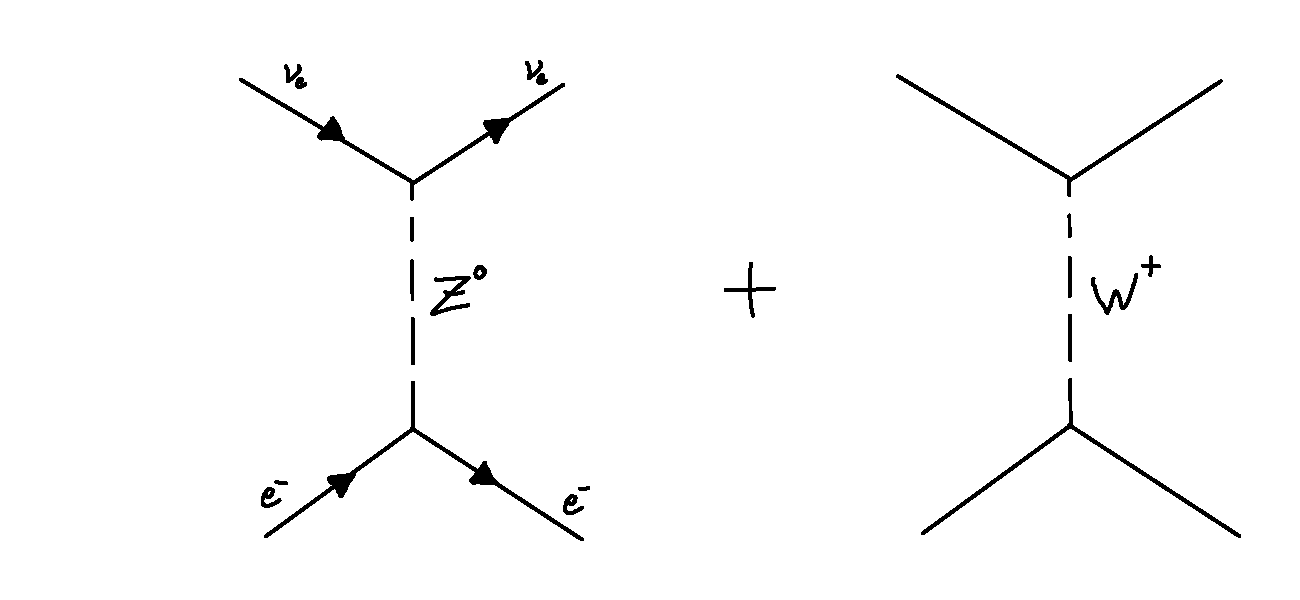
\includegraphics[width=.5\textwidth]{imgs/ep5-fig-2-5.pdf}
\caption{$Z^0$- und $W^+$-Austausch bei WW von $\nu_ee$ im Feynmandiagramm\label{fig:2.5}}
\end{figure}
$Z$-Austausch (\glqq neutral current\grqq), $W$-Austausch (\glqq charged current\grqq)\\
Propagator:
\begin{align}
\begin{split}
\sim \frac{1}{q^2 - M^2_{Z,W}}\ \Ra\ \labs M\rabs^2 \sim \frac{1}{\lb q^2 - M^2_{Z,W}\rb ^2}\\
\text{mit } \labs q^2\rabs \ll M_{Z,W}^2 \text{ folgt:}\\
\labs M \rabs ^2 \approx \frac{1}{M^4_{Z,W}}
\end{split}
\end{align}
\item \tb{Starke WW}\\
z.B. Proton-Proton-Streuung (vgl. Abb.\ref{fig:2.6})\\
\begin{figure}[!ht]
\centering
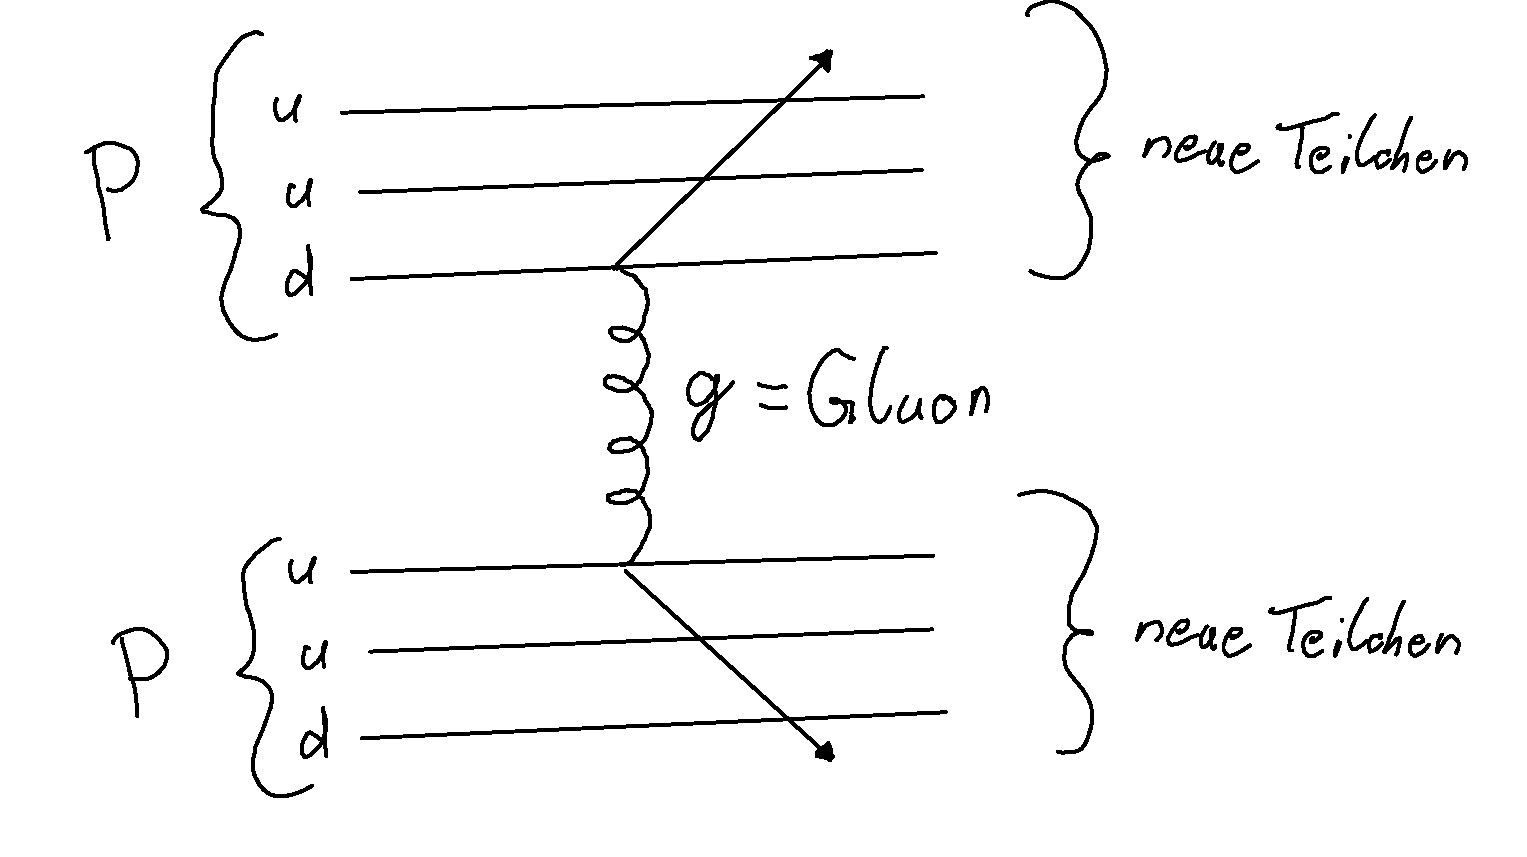
\includegraphics[width=.5\textwidth]{imgs/ep5-fig-2-6.pdf}
\caption{Gluon als Austauschteilchen bei der pp-Streuung\label{fig:2.6}}
\end{figure}
Stärke $\sim \alpha_s$ mit $\alpha_s \gg \alpha$
\end{itemize}
\end{itemize}
\section{Relative Stärke der WW, Reichweite}
Stärke der WW ist durch Kopplung und Propagator gegeben:
\begin{align}
\labs M \rabs ^2 \sim \alpha_{WW}^2 \lb  \frac{1}{q^2 - M^2_{WW}} \rb ^2
\end{align}
\begin{table}[h]
\centering
\begin{tabular}{l |c |c}
Wechselwirkung & $\alpha_{WW}$ & $M_{WW}$\\
\hline
elektromagnetische & $\alpha \approx \frac{1}{137}$ & $M_\gamma = 0$ \\
schwache & $\alpha_w \approx \frac{1}{100}$ & $M_{W,Z} = \mc{O}(100$\,GeV)\\
starke & $\alpha_s = \alpha_s\lb q^2\rb  = 0.1 \, \dots \, 10$ & $M_g = 0$
\end{tabular}
\end{table}
\tb{Beispiel:} Vergleich elektromagnetische WW mit schwacher WW (Abb.\ref{fig:2.7})\\
Kopplung ähnlich (sogar $\alpha_w > \alpha$), Propagator aber liefert:
\begin{align}
\frac{\labs M_w \rabs ^2}{\labs M_\mathrm{elm}\rabs^2} \sim \lb  \frac{q^2}{q^2 - M_Z^2}\rb ^2\ \  \overset{\labs q^2 \rabs \ll M_Z^2}{=}\ \  \frac{q^4}{M_Z^4} \ll 1
\end{align}
\begin{figure}[!ht]
\centering
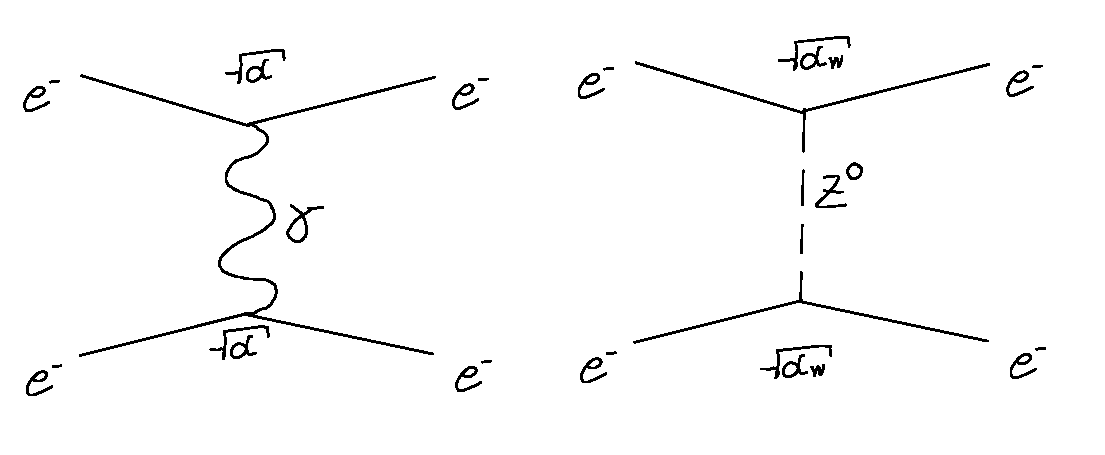
\includegraphics[width=.5\textwidth]{imgs/ep5-fig-2-7.pdf}
\caption{Feynmandiagramme zur elmag-WW (links) und zur schwachen WW (rechts)\label{fig:2.7}}
\end{figure}

\noindent\tb{Beispiel:} Vergleich elektromagnetische WW mit starker WW (Abb.\ref{fig:2.8})\\
$\ra$ Propagator gleich, aber $\alpha_s^2 \gg Z_q^2 Z_{q^\prime}^2 \alpha^2$ $\Ra$ \tb{starke WW dominiert}
\begin{figure}[!ht]
\centering
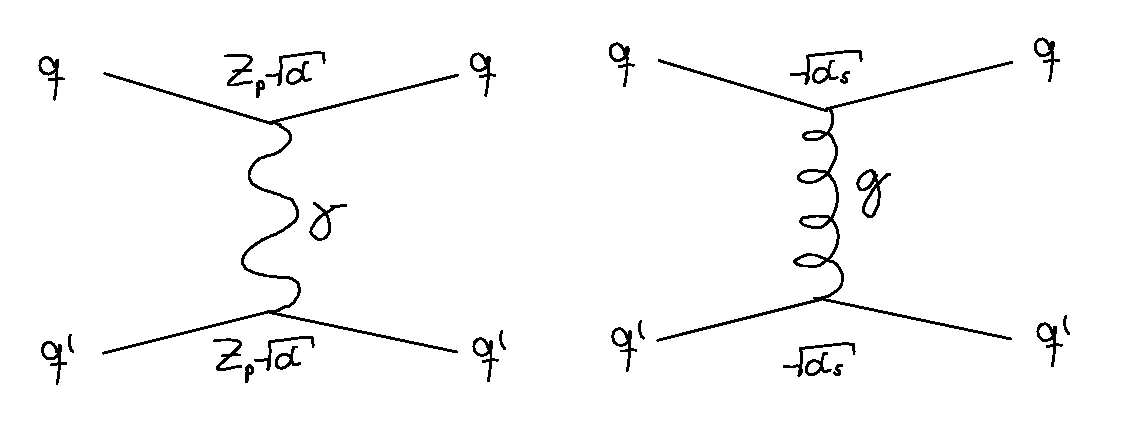
\includegraphics[width=.5\textwidth]{imgs/ep5-fig-2-8.pdf}
\caption{Feynmandiagramme zur elmag-WW (links) und zur starken WW (rechts)\label{fig:2.8}}
\end{figure}

\tb{Reichweite}\\
Die Reichweite einer WW ist \tb{kein} statisches Konzept, sondern hängt von der Dynamik ab. Sie ist dabei umso kleiner, je \glqq virtueller\grqq{} das Wechselwirkungsboson ist.
\begin{compactitem}
\item[$\ra$] elmag, starke WW: $\labs q^2 \rabs$ groß $\Ra$ Reichweite klein
\item[$\ra$] schwache WW: Bei kleinen $\labs q^2\rabs$ ist Reichweite $\sim \frac{1}{M_{Z,W}} \sim 10^{-18}$\,m
\item[$\ra$] starke WW: Abschirmung der starken Ladungen, Reichweite $\sim 10^{-15}$\,m
\end{compactitem}
\section{Raum-Zeit-Symmetrie von Wechselwirkungen}
\tb{Antiteilchen:}\\
Lösungen der Feldgleichungen zu $E<0$, die rückwärts in der Zeit laufen\\
$\Ra$ Äquivalent zu Antiteilchen mit $E>0$, die vorwärts in der Zeit laufen\\
Somit tragen Antiteilchen die \glqq umgekehrte Pfeilrichtung\grqq{} in Feynman-Diagrammen

\tb{Konsequenz:}\\
Feynmann-Diagramme \glqq können gedreht\grqq{} werden (um $n\cdot 90^\circ$) (siehe Abb.\ref{fig:2.9})

 Es fällt auf, dass einlaufende Teilchen $\leftrightarrow$ auslaufende Teilchen\\
Alle Diagramme sind erlaubt, da in jedem Fall $\labs M\rabs^2 \sim \frac{\alpha^2}{q^4}$ gilt.\\
\tb{Achtung:} Reaktionen nur erlaubt, wenn genügend Energie für Erzeugung von Endzuständen vorhanden:
\begin{align}
\begin{split}
E_\mr{CMS} > \sum_\text{Endzustand} M_i\\
q^2 = \lb E_\gamma, \vec{p}_\gamma \rb ^2; \text{ für } e^+e^- \leftrightarrow \mu^+\mu^- \text{ ist } \labs q^2 \rabs = E^2_\mr{CMS}
\end{split}
\end{align}
\begin{figure}[!ht]
\centering
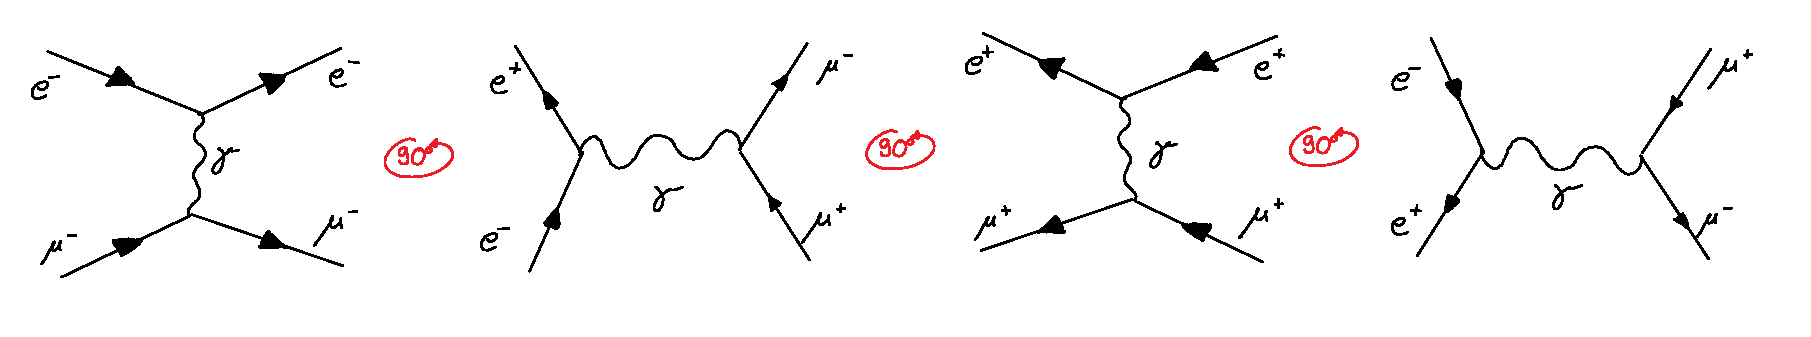
\includegraphics[width=\textwidth]{imgs/ep5-fig-2-9.pdf}
\caption{Rotation des Feynman-Diagramms von $e^-\mu^- \ra e^-\mu^-$ zu $e^+e^- \ra \mu^+\mu^-$ zu $e^+\mu^+ \ra e^+\mu^+$ und schließlich $\mu^+\mu^- \ra e^+e^-$ \label{fig:2.9}}
\end{figure}

\section{Zusammengesetzte Systeme}
\tb{In der Kern-/Teilchenphysik insbesondere:}
\begin{itemize}
\item Systeme von Quarks q
\begin{compactitem}
\item[$\ra$] $q + \bar{q}$ Meson
\item[$\ra$] $q +q +q$ Baryon
\item[$\ra$] weiter?
\item[$\Ra$] gesamt: Hadronen
\end{compactitem}
\item Atomkerne
\begin{compactitem}
\item[$\ra$] $Z\cdot p + N\cdot n$
\end{compactitem}
\item[$\Ra$] $q,p,n$: Fermionen
\item auch:
\begin{compactitem}
\item[$\ra$] Positronium ($e^+e^-$-Systeme)
\item[$\ra$] Anti-Wasserstoff $\mr{\bar{H}}\ \lb \bar{p} + e^+\rb $
\end{compactitem}
\end{itemize}

\tb{Eigenschaften zusammengesetzter Systeme}
\begin{itemize}
\item Ausgedehnt
\item Können i.A. angeregt werden wie Atome (höhere Schalen, Drehimpulse $\lt$ Spektroskopie)
\item Tragen feste Quantenzahlen: Masse $M$, Drehimpuls $L$, Spin $S$, sowie $J$ mit $\vec{J} = \vec{L}+\vec{S}$
\end{itemize}

\tb{Spin und Drehimpuls}
\begin{itemize}
\item $S$ durch Addition der Fermion-Spins: z.B. Meson mit $\ket{\frac{1}{2}} \otimes \ket{\frac{1}{2}} = \ket{0} \oplus \ket{1}$\\
$\ket{0} = \frac{1}{\sqrt{2}}\lb  \uparrow \downarrow - \downarrow \uparrow\rb $ \hfill $\ket{1,-1} = \downarrow\downarrow$ \hfill $\ket{1,0} = \frac{1}{\sqrt{2}}\lb  \ua\da + \da \ua \rb $ \hfill $\ket{1,1} = \ua\ua$
\item LS-Kopplung durch bindende WW (Achtung: starke WW bei Hadronen)\\
$\Ra$ LS-Kopplung anders als in Atomen, $\vec{J} = \vec{L} + \vec{S}$; $\labs L-S \rabs \leq J \leq L+S$
\item Notation: $n^{2s+1}L_J$, z.B. $2^3p_1$
\end{itemize}

\tb{Beispiele:}
\begin{itemize}
\item Pionen: $\pi^\pm, \pi^0$ (Mesonen) mit\\
$\pi^+ = \ket{u\bar{d}}$; $\pi^-= \ket{d\bar{u}}$; $\pi^0 = \frac{1}{\sqrt{2}} \lb  \ket{u\bar{u}} - \ket{d\bar{d}}\rb  $\\
haben $S=L=J=0$, $M_{\pi^\pm} = 139$\,MeV; $M_{\pi^0} = 135$\,MeV
\item Proton, Neutron, $\Delta$ (Baryonen) mit\\
$\ket{p} = \ket{uud}$, $M_p= 938$\,MeV, $\ket{n}=\ket{udd}$,\\
$M_n = 940$\,MeV, $\ket{\Delta^+} = \ket{uud}$, $M_\Delta = 1232$\,MeV, $p,n$\\
haben $J= \frac{1}{2}$, $ L=0$,\\
Achtung: $\Delta$ instabil: $\Delta^+ \ra \llb \begin{matrix}
p + \pi^0 \\ n +\pi^+
\end{matrix}\rno$
\end{itemize}
\section{Symmetrien und Erhaltungssätze}
\tb{Erinnerung:} Noether Theorem
\begin{framed}
\begin{center}
Invarianz eines Systems unter Symmetrieoperation $\Ra$ Erhaltungsgröße
\end{center}
\end{framed}
\begin{table}[!ht]
\centering
\begin{tabular}{l|r}
Operation & Erhaltungsgröße\\
\hline
Zeittranslation & Energie\\
Ortstranslation & Impuls\\
Drehung & Drehimpuls
\end{tabular}
\caption{Bekannte Symmetrieoperationen und deren Erhaltungsgrößen}
\end{table}
\tb{In der Teilchenphysik} treten zusätzlich diskrete Operationen bzw. Erhaltungsgrößen auf
\begin{enumerate}
\item \tb{Parität}
\begin{itemize}
\item Spiegelung der Ortskoordinaten $\ra$ Paritätsoperator $\hat{P}$ mit $\hat{P}\Psi\lb \vec{r}\rb  = \Psi \lb  -\vec{r}\rb $
\item Wenn $\Psi$ Eigenfunktion von $\hat{P}$: $\hat{P}\Psi\lb \vec{r}\rb  = \pm 1 \cdot \Psi\lb \vec{r}\rb $, wobei $\pm 1$ als Paritätsquantenzahl $P$ bezeichnet wird
\item[$\Ra$] Teilchen tragen intrinsische Parität:
\begin{align}
\begin{split}
P(\gamma) = P\lb W^\pm\rb  = P(Z) = P(g) = -1\\
P(f\bar{f}) = -1\ \lb \text{Konvention: } P(f) = +1, \ P(\bar{f}) = -1\rb 
\end{split}
\end{align}
\item Parität ist multiplikativ, z.B. System Fermion + (Anti-)Fermion:
\begin{align}
\begin{split}
\Psi\lb f_1,f_2\rb  = \Psi_1\cdot \Psi_2 \cdot \Psi\lb \vec{r}_1, \vec{r}_2\rb  \cdot \Psi \lb spin\rb \\
\Ra P\lb f_1,f_2 \rb  = P_1\cdot P_2\cdot P_r \cdot P_s\\
\Ra P\lb  q\bar{q}\rb  = -1 \cdot (-1)^L \cdot 1\\
\boxed{\Ra P\lb f\bar{f}\rb  = \lb -1\rb ^{L+1}}
\end{split}
\end{align}
\item Für System zweier Bosonen (auch z.B. $\pi^+\pi^-$)
\begin{align}
\begin{split}
P\lb B\bar{B}\rb  = (-1)^L \underbrace{(+1)}_{B\bar{B}} \underbrace{(+1)}_{s}\\
\Ra \boxed{ P\lb B\bar{B}\rb  = (-1)^L}
\end{split}
\end{align}
Wenn WW unter $\hat{P}$ invariant:
\begin{align}
\hat{P}^\dagger \Ham_{WW} \hat{P} = \Ham_{WW}
\end{align}
$\Ra$ Parität erhalten
\begin{table}[!ht]
\centering
\begin{tabular}{l|r}
WW & $P$-Erhaltung\\
\hline
elm. & \checkmark\\
stark & \checkmark\\
schwach & x (maximal verletzt)
\end{tabular}
\end{table}
\end{itemize}

\item \tb{C-Parität}\\
$\hat{C}$ = Operator der Ladungskonjugation\\
verwandelt Teilchen in sein Antiteilchen
\begin{align}
\begin{split}
\hat{C}\ket{T} = \pm \ket{\bar{T}}\\
\pm, \text{ weil } \hat{C}\hat{C}\ket{T}= \ket{T}
\end{split}
\end{align}
$\hat{C}$ ändert Ladungsvorzeichen und magnetisches Moment, lässt Masse und Spin aber invariant.\\
Eigenzustände von $\hat{C}$, falls $\ket{T}= \pm \ket{\bar{T}}$, dann
\begin{align}
\hat{C}\ket{T} = \pm \ket{T}
\end{align}
Definiere $\eta_C$ als Ladungsparität mit
\begin{align}
\eta_C (\gamma) = \eta_C ( Z^0) = -1
\end{align}
$\eta_C$ ist multiplikativ (wie $P$) für zusammenhängende Systeme:
\begin{align}
\begin{split}
\eta_C \lb  f\bar{f}\rb  = (-1)^{L+S}\\
\hat{C}\ket{f} = \pm \ket{\bar{f}}\\
\eta_C\lb B\bar{B}\rb  = (-1)^L\\
\hat{C}\ket{B} = \pm \ket{\bar{B}}
\end{split}
\end{align}
\begin{table}[!ht]
\centering
\begin{tabular}{l|r}
WW & $\eta_C$-Erhaltung\\
\hline
elm. & \checkmark\\
stark & \checkmark\\
schwach & x
\end{tabular}
\end{table}
\item \tb{CP-Symmetrie}\\
Hintereinanderausführung von $\hat{P}$ und $\hat{C}$ in schwacher WW schwach verletzt
\item \tb{T-Symmetrie}\\
$\hat{T}$: Zeitspiegelungsoperator
\begin{align}
\hat{T}\Psi \lb  \vec{r},t \rb  = \pm \Psi \lb  \vec{r}, -t\rb 
\end{align}
\item \tb{CPT-Symmetrie}
\item \tb{weitere erhaltene Größen}
\begin{itemize}
\item[$\ra$] \tb{Ladung} (elm)\\
An jedem Vertex erhalten $\ra$ Ladungserhaltung in allen WW
\item[$\ra$] \tb{Leptonzahl}
\begin{align}
\begin{split}
L\lb  e^-,\mu^-,\tau^-,\nu_e, \nu_\mu, \nu_\tau \rb  =1\\
L\lb e^+,\mu^+,\tau^+,\bar{\nu}_e, \bar{\nu}_\mu, \bar{\nu}_\tau \rb  = -1\\
L\lb  q, \gamma, W, Z, g\rb  = 0
\end{split}
\end{align}
$\ra$ in allen WW erhalten (an jedem Vertex)
\item[$\ra$] \tb{$e,\mu,\tau$-Zahl}
\begin{align}
\begin{split}
\lno \begin{matrix}
L_e \lb  e^-, \nu_e\rb  = 1\\
L_e \lb  e^+, \bar{\nu}_e\rb  = -1\\
L_e\lb \text{alle anderen}\rb  = 0
\end{matrix} \rrb\text{ analog } L_\mu, L_\tau
\end{split}
\end{align}
$\ra$ In allen WW (an allen Vertizes) erhalten. Aber: in $\nu$-Oszillation verletzt!
\item[$\ra$] \tb{Baryonzahl} -- eigentlich Quantenzahl
\begin{align}
\begin{split}
B\lb q\rb  = \frac{1}{3}\\
B\lb \bar{q}\rb  = -\frac{1}{3}\\
B\lb  p,n,\dots\rb  = 1\\B\lb  \bar{p}, \bar{n},\dots \rb  = -1\\
B\lb  \text{alle anderen}\rb  = 0
\end{split}
\end{align}
$\ra$ in allen WW erhalten
\end{itemize}
\end{enumerate}
